\documentclass[a4paper,11pt]{article}
\usepackage{amsmath,amsthm,amsfonts,amssymb,amscd,amstext,vmargin,graphics,graphicx,tabularx,multicol} \usepackage[french]{babel}
\usepackage[utf8]{inputenc}  
\usepackage[T1]{fontenc} 
\usepackage[T1]{fontenc}
\usepackage{amsmath,amssymb}
\usepackage{pstricks-add,tikz,tkz-tab,variations}
\usepackage[autolanguage,np]{numprint} 
\usepackage{color}
\usepackage{ulem}

\setmarginsrb{1.5cm}{0.5cm}{1cm}{0.5cm}{0cm}{0cm}{0cm}{0cm} %Gauche, haut, droite, haut
\newcounter{numexo}
\newcommand{\exo}[1]{\stepcounter{numexo}\noindent{\bf Exercice~\thenumexo} : \marginpar{\hfill /#1}}
\reversemarginpar


\newcounter{enumtabi}
\newcounter{enumtaba}
\newcommand{\q}{\stepcounter{enumtabi} \theenumtabi.  }
\newcommand{\qa}{\stepcounter{enumtaba} (\alph{enumtaba}) }
\newcommand{\initq}{\setcounter{enumtabi}{0}}
\newcommand{\initqa}{\setcounter{enumtaba}{0}}

\newcommand{\be}{\begin{enumerate}}
\newcommand{\ee}{\end{enumerate}}
\newcommand{\bi}{\begin{itemize}}
\newcommand{\ei}{\end{itemize}}
\newcommand{\bp}{\begin{pspicture*}}
\newcommand{\ep}{\end{pspicture*}}
\newcommand{\bt}{\begin{tabular}}
\newcommand{\et}{\end{tabular}}
\renewcommand{\tabularxcolumn}[1]{>{\centering}m{#1}} %(colonne m{} centrée, au lieu de p par défault) 
\newcommand{\tnl}{\tabularnewline}

\newcommand{\trait}{\noindent \rule{\linewidth}{0.2mm}}
\newcommand{\hs}[1]{\hspace{#1}}
\newcommand{\vs}[1]{\vspace{#1}}

\newcommand{\N}{\mathbb{N}}
\newcommand{\Z}{\mathbb{Z}}
\newcommand{\R}{\mathbb{R}}
\newcommand{\C}{\mathbb{C}}
\newcommand{\Dcal}{\mathcal{D}}
\newcommand{\Ccal}{\mathcal{C}}
\newcommand{\mc}{\mathcal}

\newcommand{\vect}[1]{\overrightarrow{#1}}
\newcommand{\ds}{\displaystyle}
\newcommand{\eq}{\quad \Leftrightarrow \quad}
\newcommand{\vecti}{\vec{\imath}}
\newcommand{\vectj}{\vec{\jmath}}
\newcommand{\Oij}{(O;\vec{\imath}, \vec{\jmath})}
\newcommand{\OIJ}{(O;I,J)}

\newcommand{\bmul}[1]{\begin{multicols}{#1}}
\newcommand{\emul}{\end{multicols}}


\newcommand{\reponse}[1][1]{%
\multido{}{#1}{\makebox[\linewidth]{\rule[0pt]{0pt}{20pt}\dotfill}
}}

\newcommand{\titre}[5] 
% #1: titre #2: haut gauche #3: bas gauche #4: haut droite #5: bas droite
{
\noindent #2 \hfill #4 \\
#3 \hfill #5

\vspace{-1.6cm}

\begin{center}\rule{6cm}{0.5mm}\end{center}
\vspace{0.2cm}
\begin{center}{\large{\textbf{#1}}}\end{center}
\begin{center}\rule{6cm}{0.5mm}\end{center}
}



\begin{document}
\pagestyle{empty}
\titre{Brevet blanc 1}{Nom}{Prénom}{Date}{Classe}
\vspace*{0.5cm}


\exo{5} QCM

Cet exercice est un questionnaire à choix multiples.\\
Pour chaque question, quatre réponses sont proposées mais une seule est exacte. Pour chacune des questions, entourer la bonne réponse, aucune justification n'est demandée.

\vspace*{0.25cm}

\renewcommand{\arraystretch}
{3.2}
\begin{flushleft}

\begin{tabular}{|p{0.75cm}|p{5cm}|c|c|c|c|}
\hline 
\textbf{N} &\textbf{ Question} & \textbf{Réponse A} & \textbf{Réponse B} & \textbf{Réponse C} & \textbf{Réponse D} \\ 
\hline 
\textbf{1} & $2 + \dfrac{2}{3} \times \dfrac{1}{4}$ est égal à & $\dfrac{13}{6}$ & $\dfrac{4}{12}$ & $\dfrac{5}{14}$ & $\dfrac{5}{7}$ \\ 
\hline 
\textbf{2} &  $\dfrac{(10^{-3})^{2} \times 10^{4}}{10^{-5}}$ est égal à :  & $10^{3}$ & $10^{-15}$ & $10^{-7}$ & $10^{4}$ \\ 
\hline 
\textbf{3} & L'écriture scientifique de 65 100 000 est & $6,51 \times 10^{7}$& $651 \times 10^{5}$ & $6,51 \times 10^{-7}$ &  $65,1 \times 10^{6}$ \\
\hline 
\textbf{4}& Soit $g(x) = x^{2} -5$. L'image de -1 par g est :& -4 & -6 & 4 & 5 \\ 
\hline 
\textbf{5} & Soit $f(x) = (x-2)(3-2x)$. L'image de 1 par g est :  & -1 & 1 & 11  & 0 \\ 
\hline 


\end{tabular} 
\end{flushleft}

\vspace*{0.25cm}

\exo{6}
Soit, ci-dessous la représentation graphique d'une fonction f.

\begin{center}
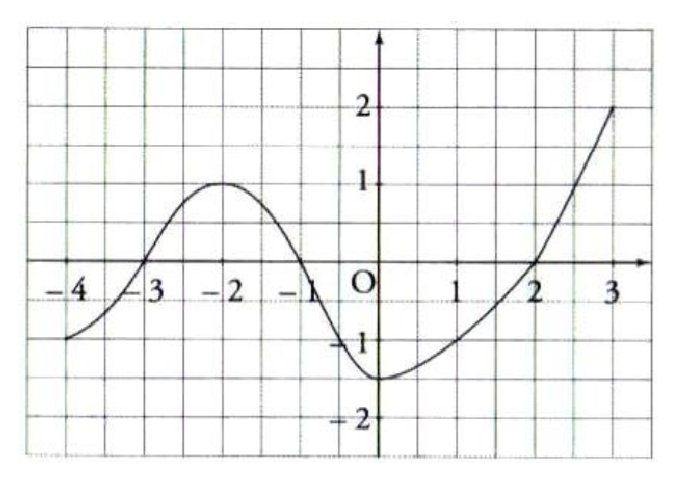
\includegraphics[scale=0.7]{exo4bb2022.eps}
\end{center}

\textit{Répondre aux questions en faisant apparaître sur le graphique les tracés nécessaires.}\\

\initq \q  Donner l'image de 0 puis celle de 1 par la fonction f.\\

\q Lire les antécédents de 1 par la fonction f.\\

\q Citer un nombre qui n'a pas d'antécédent par la fonction f.\\

\q Donner un nombre qui a trois antécédents pour la fonction f et citer ces 3 antécédents.\\

\newpage
\vspace*{0.5cm}
\exo{8}
Jean-Baptiste, élève de troisième, se promène sur l’île de Manhattan à New-York.\\

On lui a demander de vérifier que les 14ème et 42ème rues sont bien parallèles et que la 6ème avenue est bien perpendiculaires à ces deux rues.\\

Jean-Baptiste part du point C, remonte la 6ème avenue jusqu’à Bryant Park, tourne à gauche jusqu’à
Times Square, puis descend Broadway jusqu’à Union Square Park.\\

Jean-Baptiste a mesuré les longueurs suivantes :\\
CE = 1400 m, EB = 560 m, BT = 192 m,
TE = 592 m et EU = 1480 m\\


\initq \q \qa Montrer que les droites (BT) et (CU) sont parallèles.\\

\qa En déduire la distance entre le point de départ C de Jean-Baptiste et Union Square Park.\\

\q Montrer que la 14ème rue et la 6ème avenue forment un angle droit.\\

\begin{center}
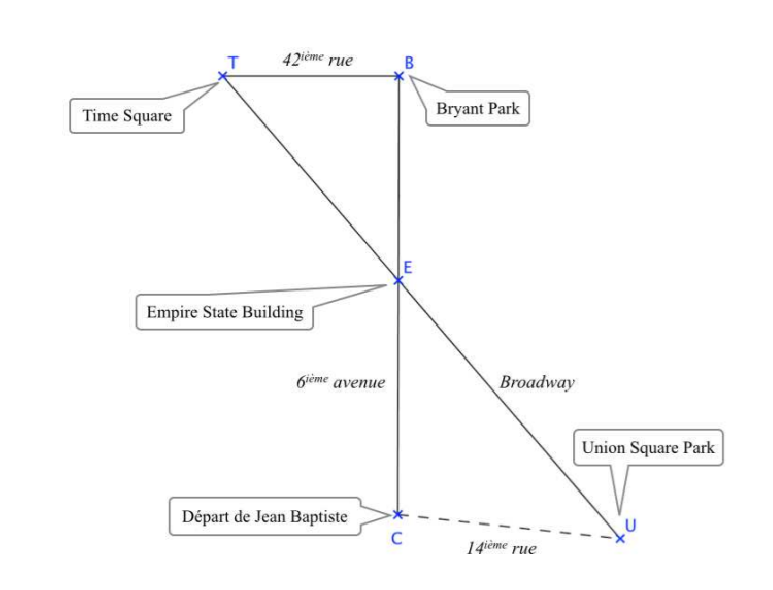
\includegraphics[scale=1]{exobb2022.eps} 
\end{center}

\newpage

\exo{9}\\


\includegraphics[scale=0.75]{exo5bb2022.eps} 

\initq \q Dans une entreprise, lors d’une visite médicale, un médecin calcule l’IMC de six des employés.
Il utilise pour cela une feuille de tableur dont voici un extrait :\\

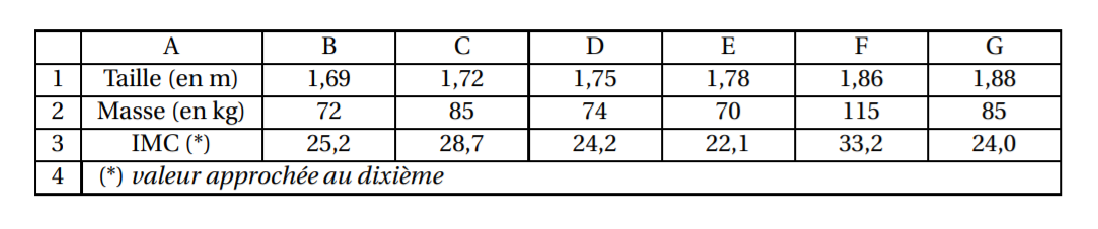
\includegraphics[scale=0.8]{exo6bb2022.eps} 

\initqa \qa Combien d'employés sont en situation de surpoids ou d’obésité dans cette entreprise ?\\

\qa Laquelle de ces formules a-t-on écrite dans la cellule B3, puis recopiée à droite, pour calculer l’IMC ?\\
Recopier la formule correcte sur la copie.\\

\includegraphics[scale=0.9]{exo7bb2022.eps}\\

 \q Le médecin a fait le bilan de l’IMC de chacun des 41 employés de cette entreprise. Il a reporté
les informations recueillies dans le tableau suivant dans lequel les IMC ont été arrondis à l’unité
près.\\
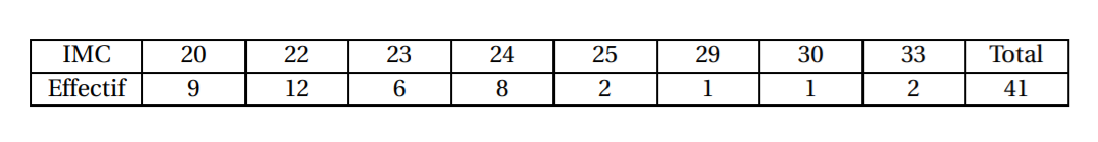
\includegraphics[scale=0.9]{exo8bb2022.eps}\\

\initqa 
\qa Calculer une valeur approchée, arrondie à l’entier près, de l’IMC moyen des employés de
cette entreprise.\\

\qa On lit sur certains magazines : « On estime qu’au moins 5 % de la population mondiale est
en surpoids ou est obèse ». Est-ce le cas pour les employés de cette entreprise ?\\

\vspace*{0.25cm}

\exo{12}\\


\includegraphics[scale=0.9]{exo2bb2022.eps} 


\initq \q Corinne choisit le nombre 1 et applique le programme A.\\
Expliquer en détaillant les calculs que le résultat du programme de calcul est 4.\\


\q Tidjane choisit le nombre -5 et applique le programme B. Quel résultat obtient-il ?\\

\q Lina souhaite regrouper le résultat de chaque programme à l'aide d'un tableur. Elle crée la
feuille de calcul ci-dessous. Quelle formule, copiée ensuite à droite dans les cellules C3 à H3,
a-t-elle saisie dans la cellule B3?\\

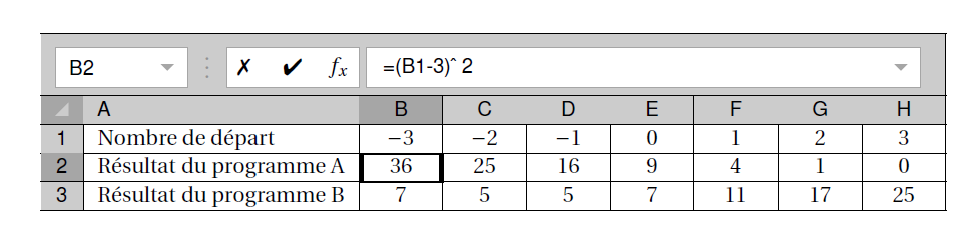
\includegraphics[scale=1]{exo3bb2022.eps} \\

\q Zoé cherche à trouver un nombre de départ pour lequel les deux programmes de calcul donnent le même résultat. Pour cela, elle appelle x le nombre choisi au départ et exprime le résultat de chaque programme de calcul en fonction de x.\\

\initqa \qa Montrer que le résultat du programme A en fonction de x peut s’écrire sous forme développée
et réduite : $x^{2} -6x +9$.\\
\qa Écrire le résultat du programme B en fonction de $x$.\\
\qa Existe-t-il un nombre de départ pour lequel les deux programmes donnent le même résultat
?
Si oui, lequel ?\\

\vspace*{0.5cm}

\exo{10} \textit{(Les transformations)}\\

\bmul{2}
\initq
\q On considère l'hexagone ABCDEF de centre O représenté ci-contre.\\
\initqa
\qa Quelle est l'image du quadrilatère CDEO par la symétrie de centre O?\\

\qa Quelle est l'image du segment [AO] par la symétrie d'axe (CF)?\\

\qa On considère la rotation de centre O qui transforme le triangle OAB en le triangle OCD.\\
Quelle est l'image du triangle BOC par cette rotation ?\\


\columnbreak

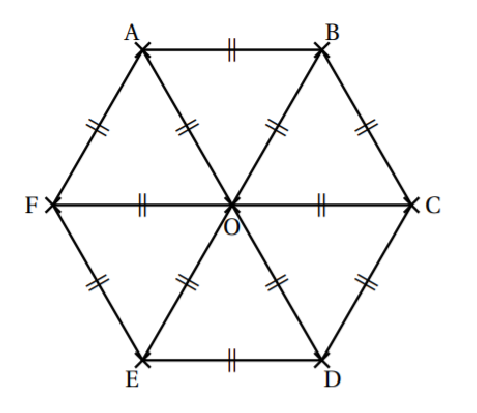
\includegraphics[scale=0.8]{hexagone1.eps} 

\emul
\vspace*{0.25cm}


\bmul{2}
\q La figure ci-contre représente un pavage dont le motif
de base a la même forme que l'hexagone ci-dessus. On
a numéroté certains de ces hexagones.\\

$\rightarrow$ \textbf{Quelle est l'image de l'hexagone 14 par la translation qui transforme l'hexagone 2 en l'hexagone
12 ?}\\

\columnbreak

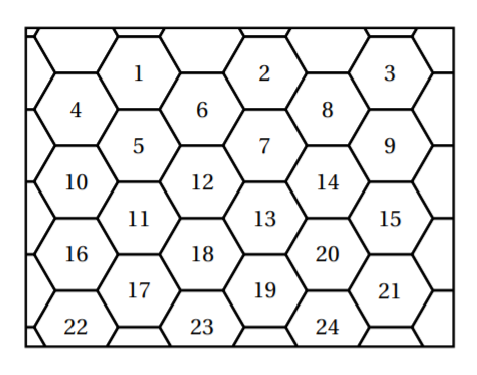
\includegraphics[scale=0.75]{nidabeille.eps} 


\emul


\end{document}
